%-*- coding: UTF-8 -*-
\documentclass[hpyerref,UTF8,a4paper,titlepage,12pt,oneside]{ctexbook}
\usepackage{hyperref}
\usepackage{geometry}
\usepackage{xeCJK, fontspec, xunicode, xltxtra,ulem}
\usepackage{amsthm}
\usepackage{amsmath}
\usepackage{amssymb}
\usepackage{mathrsfs}
\usepackage{mathtools}
\usepackage{commath}
\usepackage{listings}
\usepackage{float}
\usepackage{xcolor}
\usepackage{mdframed}

\graphicspath{{images/}}
\geometry{a4paper,bottom=2cm}

\title{PatchMatch Stereo - Stereo Matching with Slanted Support Windows}
\author{陈国庆}
\date{\today}

\bibliography{plain}

% 定理结构
\theoremstyle{definition}
\newtheorem{definition}{定义}[section]
\newtheorem{theorem}{定理}[section]
\newtheorem{corollary}{推论}[theorem]
\newtheorem{lemma}[theorem]{Lemma}
\renewcommand\qedsymbol{$\blacksquare$}

\begin{document}

\maketitle
\tableofcontents


\section{对极约束}
	如前所述,对一般场景而言,两个成像平面构不成射影变换,它们服从更一般的\textbf{极几何}约束,可用一个矩阵$F$表示这种约束关系,矩阵$F$称为\textbf{基础矩阵},
	\begin{figure}[H]
		\begin{center}
			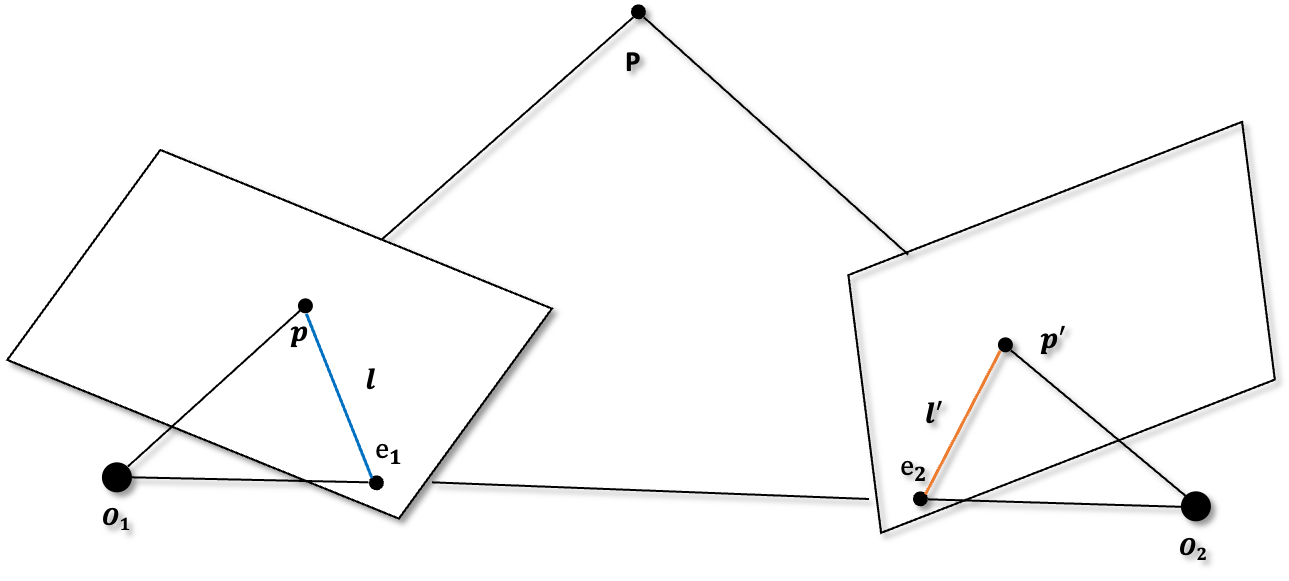
\includegraphics[width=0.8\textwidth]{../images/base_matrix.png}
		\end{center}
		\caption{两图像之间的极几何约束,$O_1,O_2$为相机\textbf{光心},$O_1O_2$为\textbf{基线},$p,p^{\prime}$为$P$在两个像素平面的像,$e,e^\prime$为\textbf{极点},$l,l^{\prime}$为\textbf{极线}}
	\end{figure}
	\begin{itemize}
		\item 世界坐标系选为第一个相机坐标系
		\item $K,K^{\prime}$是两个相机的内参矩阵
		\item $R,T$是第二个相机相对第一个相机的旋转和平移
		\item $[T]_{\times}$是$T$张成的反称矩阵,秩为$2$
		\item $e,e^\prime$为极点,$e^\prime$是$e$及原点$(0,0,0)$的投影,存在
			$$
				e^\prime = K^\prime[R \quad T]\begin{bmatrix}
					\mathbf{0}\\
					1
				\end{bmatrix} = K^\prime T
			$$	
	\end{itemize}

	所有极线都过极点,所以,
	$$
		{p^\prime}^T l^\prime = 0, \quad {e^\prime}^T l^\prime = 0
	$$
	\subsection*{基础矩阵}
		$p,p^\prime$是同一个空间点$P$在两个像素平面的投影,将$p$反投影到$P$,再投影到第二个像素平面可得到$p^\prime$,根据(\ref{inverse_proj}),

		\begin{align}
			p^{\prime}_d &= K^{\prime}[R\quad T]
			\begin{bmatrix}
				dK^{-1}p\\
				1
			\end{bmatrix}\nonumber\\
			&= K^{\prime}\left(dRK^{-1}p + T\right)\nonumber\\
			&= dK^{\prime}RK^{-1}p + K^{\prime}T\label{f_inverse}\\
			&= dK^{\prime}RK^{-1}p + e^\prime\label{f_inverse_e}
		\end{align}

		尺度因子$d$在齐次坐标下并无影响,只是提醒反投影后存在一个尺度。\\

		由此可见,一般情况下$p,p^\prime$之间并非射影变换。\\

		(\ref{f_inverse_e})式两边叉乘$e^\prime$,

		$$
			p^{\prime}_d\times e^\prime = dK^{\prime}RK^{-1}p \times e^\prime
		$$

		转置一下,
		$$
			e^\prime \times p^{\prime}_d = e^\prime \times dK^{\prime}RK^{-1}p = d[e^\prime]_{\times}K^{\prime}RK^{-1}p
		$$

		两边与$p^\prime_d$作内积,
		$$
			p^\prime_d [e^\prime]_{\times}K^{\prime}RK^{-1}p = 0
		$$

		称,
		\begin{equation*}
			\mathbf{F} = [e^\prime]_{\times}K^{\prime}RK^{-1}
		\end{equation*}

		为\textbf{基础矩阵},任意点对$p^\prime,p$都满足约束,

		\begin{equation}
			{p^{\prime}}^T \mathbf{F} p = 0 \label{f_constrain}
		\end{equation}

		根据(\ref{inver_m_p}),可得到$F$的另一表达式,

		$$
			\mathbf{F} = [e^\prime]_{\times}K^{\prime}RK^{-1} = {K^{\prime}}^{-T}[T]_{\times}RK^{-1}
		$$

		下面两个表达式都是$F$的常用形式,
		\begin{align}
			\mathbf{F} &= [e^\prime]_{\times}K^{\prime}RK^{-1} \label{f_1}\\
			\mathbf{F} &= {K^{\prime}}^{-T}[T]_{\times}RK^{-1} \label{f_1}
		\end{align}

		$[T]_{\times},[e^\prime]_{\times}$的秩为2,所以$F$的秩也为2。\\

	\subsection*{基础矩阵求解}
		基础矩阵$F$有$7$个自由度,这个点可以从两方面看出,
		\begin{itemize}
			\item \textbf{直接法},内参矩阵$K,K^\prime$已知,平移向量$T$有3个自由度,旋转矩阵$R$有4个自由度(绕某轴转某角),所以总共7个自由度
			\item \textbf{间接法},$F$是$3\times 3$矩阵,总共9个变量,一消去个不重要的尺度因子,所以总共8个变量;考虑秩为2,再消去一个变量,所以总共7个自由度
		\end{itemize}

		令$p=[x_1,x_2,1]^T,p^\prime = [x_1^\prime,x_2^\prime,1]$,

		\begin{equation}
			{p^{\prime}}^T \mathbf{F} p = 0
		\end{equation}

		可整理成,
		$$
			a\cdot f = 0
		$$

		\begin{align*}
			a &= [x_1^\prime x_2^\prime,x_1^\prime x_2,x_1^\prime, x_1x_2^\prime,x_1x_2,x_1,x_2^\prime,x_2,1]\\
			f &= [f_{11},f_{12},f_{13},f_{21},f_{22},f_{23},f_{31},f_{32},f_{33}]^T
		\end{align*}

		$a$是一对观测点$(p,p^\prime)$,$n$对点则会构成一个矩阵$D_{n \times 9}$,可构成线性方程,

		\begin{equation}\label{f_matrix_eq}
			Df = 0
		\end{equation}

		$D$称为\textbf{观测矩阵},一般通过特征匹配来确定,在SfM中属于已知量。\\

	\subsubsection*{七点法}

		一对点构造一个方程,所以7对点即可精准求解除$F$,称为\textbf{七点法}。\\

		$f$的通解为
		$$
			f = \lambda f_1 + \mu f_2
		$$

		$F$是一个齐次向量,尺度不重要,可归一化为,
		
		$$
			f = \lambda f_1 + (1-\lambda) f_2
		$$

		以及,
		$$
			F = \lambda F_1 + \mu F_2
		$$

		其中$f_1,f_2$是矩阵$D$零空间的两个基向量($D$有7个自由度,所以零空间维度为2),$F_1,F_2$为$f_1,f_2$对应的非0矩阵。\\

		因为$F$的秩为2,因此,$\det(F) = 0$,所以

		$$
			\det(\lambda F_1 + (1-\lambda) F_2) = 0
		$$

		注意$f_1,f_2,F_1,F_2$都是确定的,上面行列式展开便可求出$\lambda$,从而求出$F$。\\

		但上式展开是一个关于$\lambda$的三次函数,会得到三个根,需要排除复根和相机后面的点,从而得出正确的解。

	\subsubsection*{八点法}	
		\textbf{七点法}虽能准确求解基础矩阵,但运算过程是麻烦的,并且在实际中数据会存在噪音,只用7个点得到的解也会存在噪音。\\

		所以通常考虑多于7对点来确定基础矩阵,比如\textbf{八点法}。\\

		此时,方程(\ref{f_matrix_eq})是超定的,可转变为最小化问题,
		$$
			\min \Vert Df\Vert^2 ,\quad s.t. \quad \Vert f\Vert = 1
		$$

		这个问题变得很简单,$f$就是$D$作奇异值分解后,右奇异矩阵的最后一列。

	\subsection*{点线对应}

		$p^{\prime}$在极线$l^{\prime}$上,而$p^\prime \mathbf{F} p=0$,可知,

	\begin{align*}
		l^{\prime} = Fp,\quad 
		l = F^Tp^\prime
	\end{align*}

	基础矩阵描述了点之间的约束关系,每个点对应一条极线。\\

	极点$e^\prime$在所有极线$l^\prime$上,故,
	$$
		{e^\prime}^T l^\prime = 0 \Rightarrow {e^\prime}^TFp=0 
	$$

	因为$p$的任意性,可知

	$$
		{e^\prime}^T F = 0, \quad Fe = 0
	$$

	沿着极线$l^\prime$搜索$p$的像,会大幅缩小搜索范围。

	\subsection*{工程实现}
		在实际计算时,通过投影矩阵的增广的投影矩阵表示更为方便,
		\begin{equation}
			N_d= M^{\prime}M^{-1} = \begin{bmatrix}
				dK^\prime R K^{-1} \quad& K^\prime T\\
				0\quad& 1\quad
			\end{bmatrix}\label{extend_f}		
		\end{equation}

		从$N_d$中截取出左上角$3\times 3$的矩阵便是旋转矩阵,右上角$3\times 1$的向量是平移向量,这在各种工具中非常容易实现。

\section{外参恢复}\label{section_recovery_outer_p}
	基础矩阵$F$包含了相机的内外参数,如果相机内参已知,能否从$F$中分离出外参?\\

	$$
		\mathbf{F} = {K^{\prime}}^{-T}[T]_{\times}RK^{-1} \Rightarrow {K^{\prime}}^{T}\mathbf{F} K = [T]_{\times}R = \mathbf{E}
	$$

	其中,
	$$
		\mathbf{E} = [T]_{\times}R
	$$

	称为\textbf{本质矩阵}。现在问题简化为如何从$E$中分离出外参$R,T$。\\

	根据(\ref{inverse_decompose}),$[T]_{\times}$可分解为,

	\begin{align*}
		[T]_{\times} &= U diag(1,1,0)WU^T\\
		[T]_{\times} &= U diag(1,1,0)W^TU^T
	\end{align*}

	这两种分解仅差一个尺度或者符号。$E$可表示为,

	\begin{align*}
		\mathbf{E} = U diag(1,1,0)\left(WU^TR\right)\quad 
		\text{or} \quad 
		U diag(1,1,0)\left(W^TU^TR\right)
	\end{align*}

	注意$E$是秩为2的反称矩阵,奇异值分解形式为,

	$$
		\mathbf{E} = U diag(1,1,0) V^T
	$$

	在$\mathbf{E} $确定的情况下,$U,V$是已知量,对比可知,
	\begin{align*}
		V^T = WU^TR \quad \text{or}\quad W^TU^TR
	\end{align*}

	得到$R$的两种表达式,
	\begin{align*}
		R = UW^TV^T\quad \text{or}\quad UWV^T
	\end{align*}

	$R$是旋转矩阵,所以行列式值为正,修正一下符号,

	$$
		R \leftarrow (\mathop{det} R)R
	$$

	而,
	$$
		[T]_{\times} = R^T\mathbf{E}
	$$

	这样得到$T$的反称矩阵,可以组合出$T$向量;$R$有两个值,$T$也对应有两个值。\\


	这两组解几何表示,一组场景都在相机前面;一组场景在相机后面,通过重建出的点过滤掉在后面的解即可。

\section{单应变换}

	如果拍摄场景是一张平面,法向量为$\mathbf{n}$,到原点距离为$d$,则平面方程为,
	$$
		\mathbf{n}^T P = d
	$$

	$\mathbf{n}_d = \mathbf{n}/d$,场景平面可表示为,
	
	$$
		\mathbf{n}_d^T P = 1
	$$

	像素点$p$反投影为$dK^{-1}p$,

	\begin{align*}
		p^{\prime}(d) &= K^{\prime}\left(dRK^{-1}p + T\right)\\
		&= K^{\prime}\left(dRK^{-1}p + T\mathbf{n}_d^T P\right)\\
		&= K^{\prime}\left(dRK^{-1}p + T\mathbf{n}_d^TdK^{-1}p\right)\\
		&= dK^{\prime}\left(R + T\mathbf{n}_d^T\right)K^{-1}p\\
		&= Hp
	\end{align*}

	这里的关键是第二步,代入场景平面方程,把$p$给分离了出来,$p^\prime,p$之间构成射影变换。\\

	$K^\prime$是齐次矩阵,与$dK^\prime$等价。

	\begin{equation}
		H= K^{\prime}\left(R + T\mathbf{n}_d^T\right)K^{-1} \label{homograph_matrix}
	\end{equation}

	称为\textbf{单应矩阵},因此射影变换也称为\textbf{单应变换}。\\

	$p,p^{\prime}$依然服从基础矩阵的约束,(\ref{extend_f})式的增广表示也包含了单应变换这一特殊情况。\\

	基础矩阵只是描述点与极线的对应关系,而单应矩阵描述点之间一一对应关系,这也是“\textbf{单应}”的意义。

	\subsection*{论文中的公式}

	在MVSNet中,只知道两个相机在世界坐标系的旋转和平移$R_1,t_1,R_2, t_2$,相对旋转$R$和平移$t$为,

	$$
		R = R_2R_1^{-1},\quad 
		t = t_2 - R_2R_1^{-1}t_1
	$$

	(\ref{homograph_matrix})用世界坐标系可表示为,

	\begin{align}
		H &= K_2 \left(R_2R_1^{-1} +\left(t_2 - R_2R_1^{-1}t_1\right) \mathbf{n}_d^T\right) K_1^{-1} \label{new_homograph_matrix}
	\end{align}	

	原论文中的公式是错误的,这是正确版本。\\

	增广表示蕴含了单应变换,这个复杂的式子在编程中并不会被使用到。
\section{SfM}
	\definition{SfM问题} 也称为\textbf{欧式结构恢复问题},已知$m$张图片和对应的相机内参矩阵$K_i(i=1,\cdots,m)$,求解:
	\begin{itemize}
		\item \textbf{Structure}:$n$个三维点$X_j(j=1,\cdots\,n)$的坐标
		\item \textbf{Motion}:$m$个相机的外参数$R_i,T_i(i=1,\cdots,m)$
	\end{itemize}		
	
	如果没有额外信息,无法恢复出场景的绝对坐标(经纬度)、朝向及尺度,恢复的最好结果是与真实场景之间差一个相似变换;\\

	比如,如果知道场景中某两点之间的真实距离,则可恢复出场景的尺度,但依然无法确定绝对坐标和朝向。

	\subsection{平行视图}
		在传统两视图(\ref{two_stereo})重建场景,两个相机只有平移而无旋转,此时$R = \mathbf{I}$,基础矩阵可简化为,
		$$
			\mathbf{F} = [e^\prime]_{\times}K^{\prime}K^{-1}
		$$

		一般两个相机会采用相同的参数,此时$K = K^\prime$,基础矩阵可进一步简化为,
		$$
			\mathbf{F} = [e^\prime]_{\times}
		$$

		平行视图的场景,极点为无穷远点,极线都平行于基线,此时$e^\prime = (1,0,0)^T$,

		$$
			\mathbf{F} =  \begin{bmatrix}
				0\quad & 0\quad& 0\\
				0\quad & 0\quad& -1\\
				0\quad & 1\quad& 0
			\end{bmatrix}
		$$

		根据(\ref{f_inverse_e}),
		\begin{equation}
			p^\prime_d = dp + e^\prime = d(u+1/d,v,1)^T \label{disparity_pair}
		\end{equation}

		此时,$p^\prime_u = u + 1/d, p^\prime_v = v$,即对应点的$v^\prime$坐标与原$v$坐标坐标是相同的,两条极线具有相同的高度,此时极线也称为\textbf{扫描线}。

		\begin{figure}[H]
			% \begin{center}
			\begin{minipage}[t]{0.49\linewidth}
				\centering
				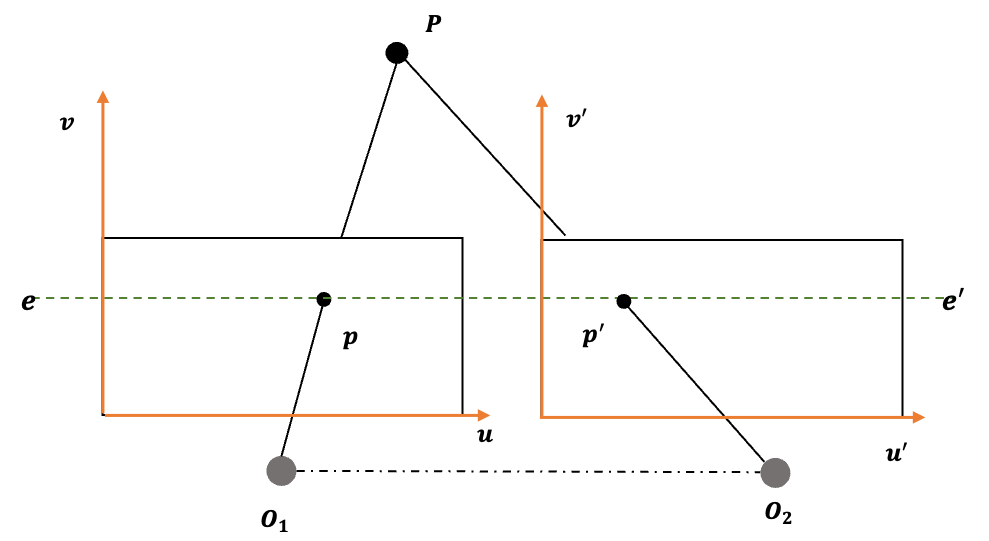
\includegraphics[width=\textwidth]{../images/two_stereo.png}
				\caption{平行视图}
				\label{two_stereo}
			\end{minipage}
			\begin{minipage}[t]{0.49\linewidth}
				\centering
				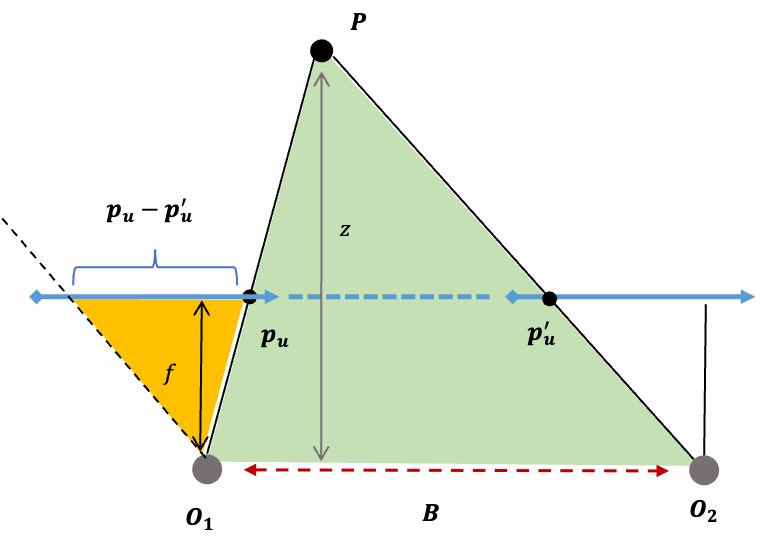
\includegraphics[width=\textwidth]{../images/two_stereo_depth.png}
				\caption{平行视图俯视几何}
				\label{two_stereo_gemotry}
			\end{minipage}			
		\end{figure}

		沿着扫描线,平行视图的深度计算非常容易,如图(\ref{two_stereo_gemotry})两个三角形相似,可得,
		$$
			p_u - p^\prime_u = \frac{Bf}{z}
		$$

		$p_u - p^\prime_u$称为\textbf{视差},是同一3D点在两个成像平面的水平像素差。$B,f$均为已知量,以此知视差与深度成反比。

		\subsubsection*{极线校正}
			上面说的平行视图是非常理想的情况,实际上之前提到过,因为工艺的原因,很难保证单相机的像平面是矩形,也很难保证两个相机的像平面是绝对平移的;\\

			对此需要将两个像平面修正为平行平面,此时极线才能真正构成\textbf{扫描线},这个过程称为\textbf{极线校正}。具体来说,先把第二个平面的极点$e^\prime$变换到$(1,0,0)^T$,得到变换矩阵$H^\prime$;再利用投影误差最小化,得到第一个平面的变换矩阵$H$,如此可使得两极线对齐。具体细节请参考鲁鹏老师课程。
			\begin{figure}[H]
				\begin{center}
					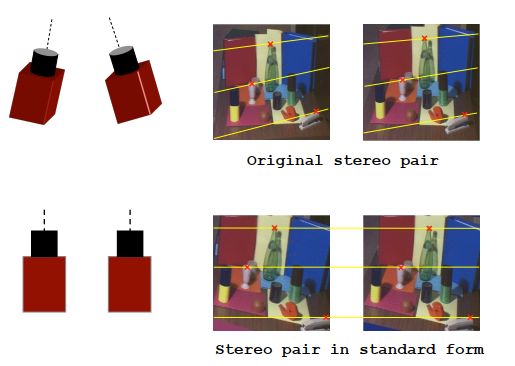
\includegraphics[width=0.8\textwidth]{../images/epipolar.png}
				\end{center}
				\caption{极线校正}
			\end{figure}

		\subsubsection*{Matching Cost}
			根据(\ref{disparity_pair}),

			$$
				p_u - p^\prime_u = \frac{1}{d}
			$$

			视差与反投影距离$d$成反比,针对某个具体的点$p$,此处的$d$是某个确定的值$d_0$;\\

			不同的$d$会产生不同的视差,给$d$一个范围,逐一计算视差范围内的代价,每一代价$c_i$对应$p_i^\prime$。\\

			$w\times h$的图片,会产生$w\times h\times d$的的张量,称为\textbf{匹配代价},MVSNet的的\textbf{Cost Volume}实际是将这一概念从两视图推广到了多视图。\\

			\begin{figure}[H]
				\begin{center}
					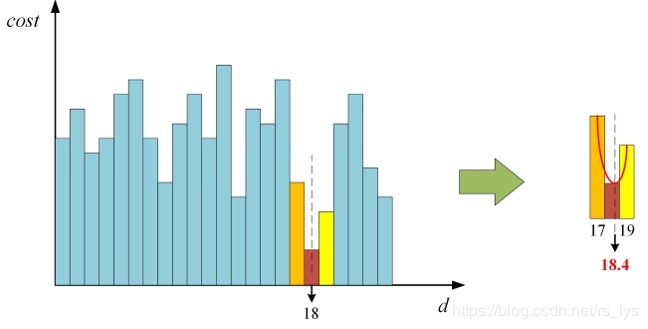
\includegraphics[width=0.85\textwidth]{../images/matching_cost.jpeg}
				\end{center}
				\caption{Matching Cost \& 二次曲线修正\protect\footnote{\url{https://blog.csdn.net/rs_lys/article/details/83302323}}}
			\end{figure}

			那些平行于像平面的场景点深度是相同的,产生的视差也是相同的,这样的平面称也为\textbf{fronto-parallel}平面;\\

			而场景中的斜面(\textbf{slanted plane}),虽然也是平面,但上面点的深度是不同的,所以产生的视差也是不同的。\\

			在计算匹配代价时,像素视差误差会平方放大深度误差($d$为视差,$D$为深度),

			$$
				\Delta d= -\frac{Bf}{D^2}\Delta D \Rightarrow \Delta D = -\frac{D^2}{Bf}\Delta d
			$$
			
			所以需要通过视差变化来刻画点对之间的匹配程度,比如,视差变化很小的区域可能处在同一\textbf{fronto-parallel}平面;视差变化连续的区域可能处在同一\textbf{slanted plane}上;而视差变化剧烈的区域可能处在不同的曲面或曲率很大的曲面上。\\

			这是各种文献里都要对fronto-parallel plane、slanted plane及其他情况进行区分的原因。

		\subsubsection*{双目立体匹配}
			双目立体成本较低,一般用在自动驾驶或机器人场景,传统的匹配过程包括四个步骤:

			\begin{enumerate}
				\item 代价计算,具体就是衡量在两张图像上点对的匹配代价,代价可以是两点灰度绝对值差、绝对值和、归一化相关系数、互信息、Census变换、Rank变换等方法衡量;对匹配范围而已,主要是局部计算,可以点点计算,也可邻域匹配计算
				\item 代价聚合,通过局部或者全局的方式进一步调优上一步的匹配代价
					\begin{itemize}
						\item 局部方法,通过\textbf{支撑窗口}做均值滤波,又分为固定窗和自适应窗
						\item 全局方法,定义一个能量函数,最小化整体点点代价匹配,转化为一个优化问题
					\end{itemize}
				\item 视差计算,取代价最小的视差作为真值
				\item 视差优化,手段包括提高精度,比如上图通过二次曲线拟合将视差整数值扩展到浮点值;剔除错误匹配、弱纹理优化、填补空洞等
			\end{enumerate}

			最为提及的概念便是局部方法中的\textbf{support window},实际就是一个常见的邻域均值,以此抑制单点噪音。\\

			但窗内的像素可能因深度不同而导致视差不同,固定窗的均值滤波可能会因此引入视差噪音,从而放大深度误差,因此有一些自适应窗的方法来应对这个问题,这里不再展开。\\

			实际上,全局方法和局部方法一样,也暗含了邻域视差不变的假设\footnote{\url{http://vision.deis.unibo.it/~smatt/Seminars/StereoVision.pdf}}。


	\subsection{两视图重建}

	考虑两张图片,只要能估计出基础矩阵$F$,便可根据\ref{section_recovery_outer_p}节估计出$R,T$,
	$$
		p^\prime F p = 0
	$$

	根据基础矩阵约束,$p=(u,v,1)^T,p^{\prime} = (u^{\prime}, v^{\prime},1)$
	$$
		(u^{\prime}, v^{\prime},1)
		\begin{bmatrix}
			F_{11}\quad& F_{12}\quad& F_{13}\\
			F_{21}\quad& F_{22}\quad& F_{23}\\
			F_{31}\quad& F_{32}\quad& F_{33}\\
		\end{bmatrix}
		(u,v,1)^T = 0
	$$
	展开可得,

	$$
		\left(uu^{\prime}, vu^{\prime}, u^{\prime}, uv^{\prime},vv^{\prime},v^{\prime},u,v,1\right)
		\begin{bmatrix*}
			F_{11}\\
			F_{12}\\
			F_{13}\\
			F_{21}\\
			F_{22}\\
			F_{23}\\
			F_{31}\\
			F_{31}\\
			F_{33}
		\end{bmatrix*} = 0
	$$

	在不考虑尺度的情况下,$F$矩阵有8个未知数,因此至少需要8对点才能确定$F$,实际上会用大于8对点,求一个最小二乘解。\\

	$F$的秩为2,最小二乘解得到的矩阵秩一般为3,需要做一次SVD分解,置最小特征值为0,来得到$F$。

	\subsubsection*{解的存在性}
		并不是任意8对点都能求解出$F$,如果8个方程中部分线性相关,会导致方程的数量少于未知数的数量,从而没有唯一解。\\

		如果场景是一张平面,$P_i(i=1,2,3)$是平面上不共线的三点,对应像素坐标$p_i,p^\prime_i$;

		平面上任意点$P$可表示为$P_i$的线性组合,$P=\alpha P_1 + \beta P_2 + \gamma P_3$,$P$的投影为,
		
		\begin{align*}
			p &= K\left(\alpha P_1 + \beta P_2 + \gamma P_3\right)\\
				&= \alpha KP_1 + \beta K P_2 + \gamma KP_3\\
				&= \alpha p_1 + \beta p_2 + \gamma p_3
		\end{align*}

		同理,
		$$
			p^\prime = \alpha p_1^\prime + \beta p_2^\prime + \gamma p_3^\prime
		$$

		因此,点对$(p,p^\prime)$贡献了一个冗余方程,或者说不影响线性方程组矩阵的秩,此时基础矩阵没有唯一解。\\

		实际上要使得线性无关的方程数量至少为8,方程才有唯一解。\\

		在单应变换的情况下,需求解单应矩阵,单应矩阵包含了基础矩阵所有的元素,以此来构造基础矩阵。\\

		为了避免陷入讨论解的存在性,在重建场景时,经常用基础矩阵和单应矩阵分别求解一次,哪个效果好用哪个。

	\subsubsection*{确定对应点对}
		怎么确定两张图像的对应点对$p,p^{\prime}$?可以用传统的SIFT特征匹配,也可以用深度学习的方法,这里就不再详细介绍。

	
	注意这里世界坐标系选择为第一个相机的坐标系,因此只有第二个相机的$R,T$需要求解,得到基础矩阵$R,T$后,根据投影关系,
	$$
		P_d = dK^{-1}p
	$$

	可计算出空间点$P$的3D坐标,也称点云,这就是\textbf{三角化}方法。\\

	这个坐标是在第一个相机坐标系下的坐标,并且重建出的目标会跟真实大小相差一个尺度$d$。

	\subsection{多视图重建}
		多张图片,多个相机内参矩阵,求解SfM问题常用\textbf{增量法},具体来说包括几个步骤,
	
	\begin{itemize}
		\item 相机之间通过两视图方法两两求解$F_{ij}$
		\item 从一对相机开始,不断加入其他相机,这样重建的点会越来越多
		\item 持续加入相机会累积误差,所以通过\textbf{捆绑调整}(Bundle Adjustment)来做一个整体优化
	\end{itemize}

	其中细节和技巧非常多,具体请参考鲁鹏老师的课程\footnote{\url{https://www.bilibili.com/video/BV1Ss4y197CU}}(多视图重建一节)。\\

	这里要说的是这个\textbf{捆绑调整}方法,本质通过$L_2$距离最小化投影误差,
	$$
		E(M,X) = \sum_{i=1}^m \sum_{j=1}^n D\left(x_{ij}, M_iX_j\right)^2
	$$

	\begin{figure}[H]
		\begin{center}
			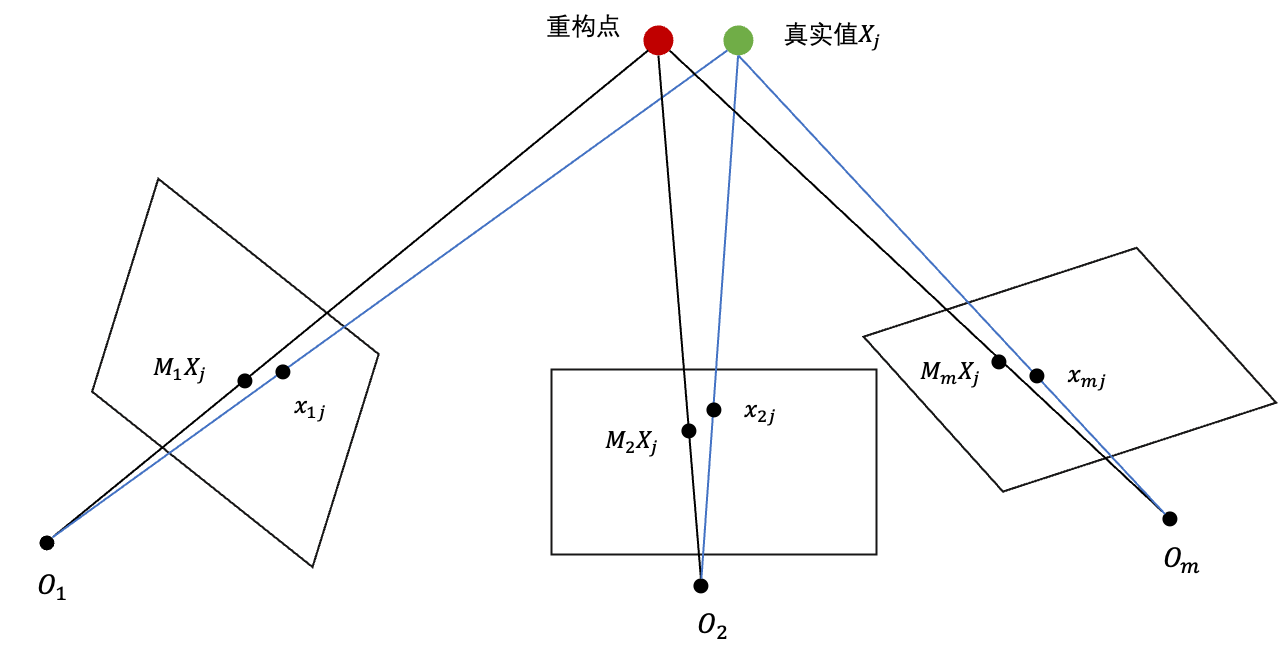
\includegraphics[width=\textwidth]{../images/ba.png}
		\end{center}
		\caption{BA重投影误差}
	\end{figure}

	理论上可以通过梯度下降优化BA,直接得到$M,X$;实际上传统做法是先用增量法求的一个初解,再用BA方法优化,以加速收敛。\\

	如果样本足够多,将传统SfM转化为机器学习问题,效果也未必就差;但传统方法是对单场景重建,能收集的样本有限。\\

	图像上的点,至少被两个相机看到,构成点对的点才能计算出深度信息,如果两个相机姿态差距太大,会因为遮挡等原因导致可匹配的点减少。\\

	BA优势就是不需要所有的点都被所有的相机看到,每个相机只关注自己能看到点即可。
\section{MVSNet}

	不同于传统的SfM估计一次优化能得到整个场景的点云,MVSNet\footnote{\url{https://arxiv.org/abs/1804.02505}}只是推断每张图片的深度信息,通过后处理,把多张图片的深度,拼成场景点云。\\

	主要思路是通过2张目标图来协助推断参考图的深度值,

	\begin{enumerate}
		\item 把参考相机(第一个相机)像素平面的坐标,通过192个尺度反投影到相机坐标系;然后通过单应矩阵变换到目标相机的像素坐标系。

		\small\textit{ 注意,这里的变换对象是参考相机的$120 \times 160$像素平面坐标,而非论文说的参考图像的特征图;}

		经过这步操作,可在目标相机的像素平面上形成192个$120 \times 160$的新的像素坐标值。

		\item 把投影得到的像素坐标值与目标图像的特征图结合,得到192个目标特征图

		\small\textit{把192个特征图按深度叠在一起,形成一个$192 \times 120 \times 160 \times 32$的特征图,称为\textbf{Feature Volume}}

		\item 把多个(文中为2个)目标\textbf{Feature Volume}连同参考图像的特征图一起,计算一个方差,得到的结果称为\textbf{Cost Volume},随后在\textbf{Cost Volume}上回归参考图像的深度值

		\small\textit{注意,此时才用到参考图像的特征图}
	\end{enumerate}

	\begin{figure}[H]
		\begin{center}
			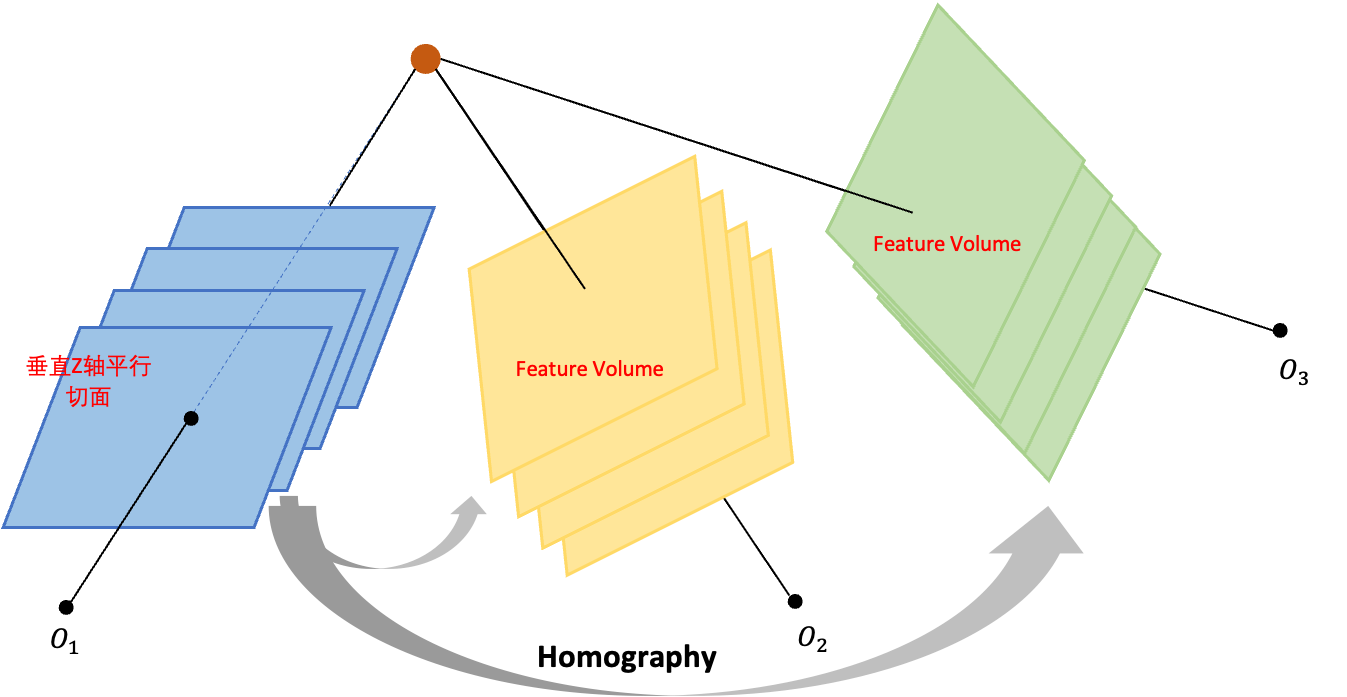
\includegraphics[width=\textwidth]{../images/fronto.png}
		\end{center}
		\caption{相机1将场景按深度切片称为\textbf{Fronto parallel},分别投影到相机2,3像素平面,形成\textbf{Feature Volume}}
	\end{figure}

\subsection{目标相机的作用}

	目标相机对预测参考图像的深度有什么帮助?我是这么认为的,因为世界坐标系选为参考相机的坐标系,如果参考图像上有一个点深度为$d$,那么其他相机看到这个点深度也应该为$d$,也就是用目标图像的特征预测出的深度也应该为$d$。\\

	因此,如果一个点的深度在各个相机下预测正确,那么方差就会很小,否则方差会变大,这是作者认为\textbf{Cost Volume}有作用的原因。\\

	把\textbf{Feature Volume}的平均作为回归目标也是可行的,但作者在消融实验提到效果不如方差,这里是个玄学。\\

	提升目标图片数量,预测效果也会提升,作者实验过5张图片效果好于2张。能提升预测效果的图片是那些与目标相机姿态差距不是很大的图片,所以这个数量也是有上限的。

\subsection{单应变换的作用}
	MVSNet工作重点便是单应变换,主要体现在:
	\begin{itemize}
		\item 通过单应变换把场景切面变换到目标相机像素坐标系
		\item 单应变换可求导,使得变换过程可训练
	\end{itemize}

	然而,变换切面通过增广矩阵的逆变换即可,矩阵变换本身可求导,顺便包含了第二点。\\

	虽然全文都在介绍单应矩阵,实现实际完全不需要这个概念,更不需要那些复杂的推导,是不是有点讽刺!\\

	需要考虑下面两个问题,对单应变换的影响,
	\begin{itemize}
		\item 不同深度的切面通过单应变换产生的像素值会有多大的差异?
		\item 单应变换产生的新坐标如何跟目标特征图结合生成新的特征图?
	\end{itemize}

	\subsubsection*{深度对像素坐标的影响}
	对第一个问题,单应矩阵$H$可以简化为,

	\begin{align*}
		H_d= K^{\prime}\left(R + T\mathbf{n}_d^T\right)K^{-1} &= \mathbf{A} +\frac{1}{d}\mathbf{B}\\
		&= \begin{bmatrix}
			\mathbf{A}_1 + \frac{1}{d}\mathbf{B}_1\\
			\mathbf{A}_2 + \frac{1}{d}\mathbf{B}_3\\
			\mathbf{A}_3 + \frac{1}{d}\mathbf{B}_4
		\end{bmatrix}
	\end{align*}

	$\mathbf{A}=K^\prime R K^{-1},\mathbf{B}=K^{\prime}T\mathbf{n}^TK^{-1}$,只有$d$是变量,
	$$
		p^\prime(d) = H_d p = \begin{bmatrix}
			\left(\mathbf{A}_1 + \frac{1}{d}\mathbf{B}_1\right)p\\
			\left(\mathbf{A}_2 + \frac{1}{d}\mathbf{B}_3\right)p\\
			\left(\mathbf{A}_3 + \frac{1}{d}\mathbf{B}_4\right)p
		\end{bmatrix}
	$$

	$p^\prime$的欧式坐标$p^\prime_e$为,
	$$
		p^\prime_e(d) = \left(
			\frac{\left(\mathbf{A}_1 + \frac{1}{d}\mathbf{B}_1\right)p}{\left(\mathbf{A}_3 + \frac{1}{d}\mathbf{B}_3\right)p},
			\frac{\left(\mathbf{A}_2 + \frac{1}{d}\mathbf{B}_3\right)p}{\left(\mathbf{A}_3 + \frac{1}{d}\mathbf{B}_3\right)p}
		\right)^T
	$$

	$$
		p^\prime_e(\infty) = \lim_{d\rightarrow \infty}p^\prime_e(d) = \left(
			\frac{\mathbf{A}_1p}{\mathbf{A}_3p},
			\frac{\mathbf{A}_2p}{\mathbf{A}_3p}
		\right)^T
	$$

	$$
		p^\prime_e(0) = \lim_{d\rightarrow 0}p^\prime_e(d) = \left(
			\frac{\mathbf{B}_1p}{\mathbf{B}_3p},
			\frac{\mathbf{B}_2p}{\mathbf{B}_3p}
		\right)^T
	$$	

	深度$d$的确影响投影的$u,v$坐标,且输出在$p^\prime_e(0)$和$p^\prime_e(\infty)$之间。\\

	但因为在两端存在极限,所以$d$在一定的区间内变化,对$u,v$才能有显著的影响,
	
	\subsubsection*{变换特征映射}
		现在考虑第二个问题,参考相机和目标相机像素平面分辨率为$120 \times 160$,超出这个区间的变换坐标怎么处理?\\

		MVSNet的是根据最大坐标值,$u^\prime = u/119, v^\prime = v/159$(坐标从0开始)后变换到$[-1,1]$,对超出此区间的坐标一律忽略。\\

		目标特征图的左上角对应$(-1,-1)$,右下角对应$(1,1)$,根据$(u^\prime, v^\prime)$的值查找特征图上对应的点(连续值),并根据周围四个坐标(离散值)做双线性插值计算具体对应值。\\

		显然,考相机和目标相机的分辨率即使不同,也不影响这个插值过程。\\

		如果超出$(120,160)$的坐标都被忽略,是否会降低学习效果?\\

		这里实际隐含一个约束,要求两个相机应该能看到尽量多的共同点,这通过图像对的选择策略来实现,称为\textbf{视角选择}。

\subsection{视角选择}
	
	\begin{figure}[H]
		\begin{minipage}[t]{0.48\linewidth}
			\centering
			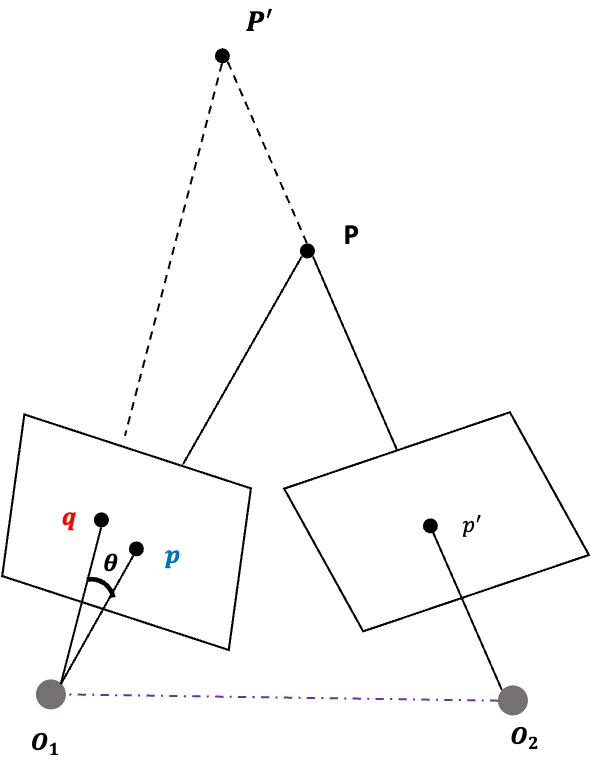
\includegraphics[width=\textwidth]{../images/baseline_error.png}
			\caption{基线太小,重建误差较大}
		\end{minipage}		
		\begin{minipage}[t]{0.52\linewidth}
			\centering
			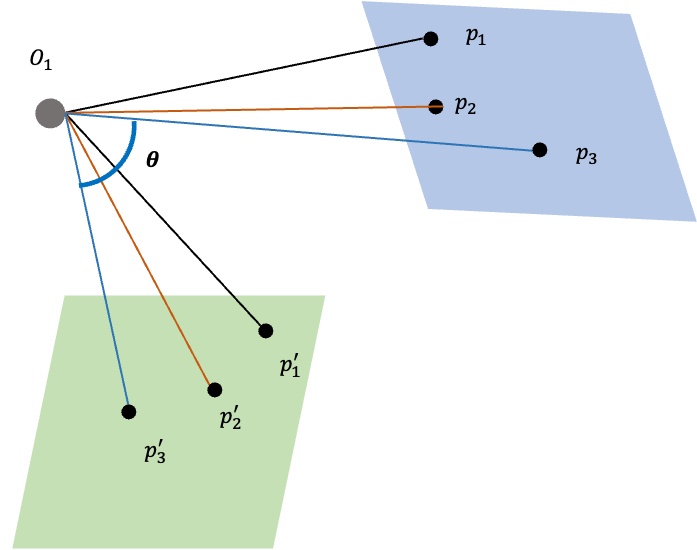
\includegraphics[width=\textwidth]{../images/track_filter.png}
			\caption{通过Track过滤小基线视角}
		\end{minipage}			
	\end{figure}

	图一小基线的场景,如果$p^\prime$误匹配$q$,$p,q$虽然只偏离了一个小角度$\theta$,重建的$P^\prime$与$P$误差也很大。\\

	反之,大基线场景会产生遮挡,极大减少可重建点数。MVSNet给出下面的评分机制来选择合适的图像对,

	$$
		\theta_{ij} = (180/\pi)\arccos\left(
			(\mathbf{c}_i - \mathbf{p})
			\cdot
			(\mathbf{c}_j - \mathbf{p})
		\right)
	$$

	$\theta_{ij}$为点对夹角,计算方法是:将像素坐标投影回世界坐标系,以第一个相机的光心为原点计算内积的反余弦(图二);\\

	\textit{相机内参和像素坐标都已知,这个过程是没问题的。}\\

	通过下面分段函数把$\theta_{ij}$拟合为打分,

	$$
		\mathcal{G}(\theta) = 
		\begin{cases}
			\exp\left(
				-\frac{(\theta-\theta_0)^2}{2\sigma_1^2}
			\right), \theta \leq \theta_0\\
			\exp\left(
				-\frac{(\theta-\theta_0)^2}{2\sigma_2^2}
			\right), \theta > \theta_0\\
		\end{cases}
	$$

	\begin{figure}[H]
		\begin{center}
			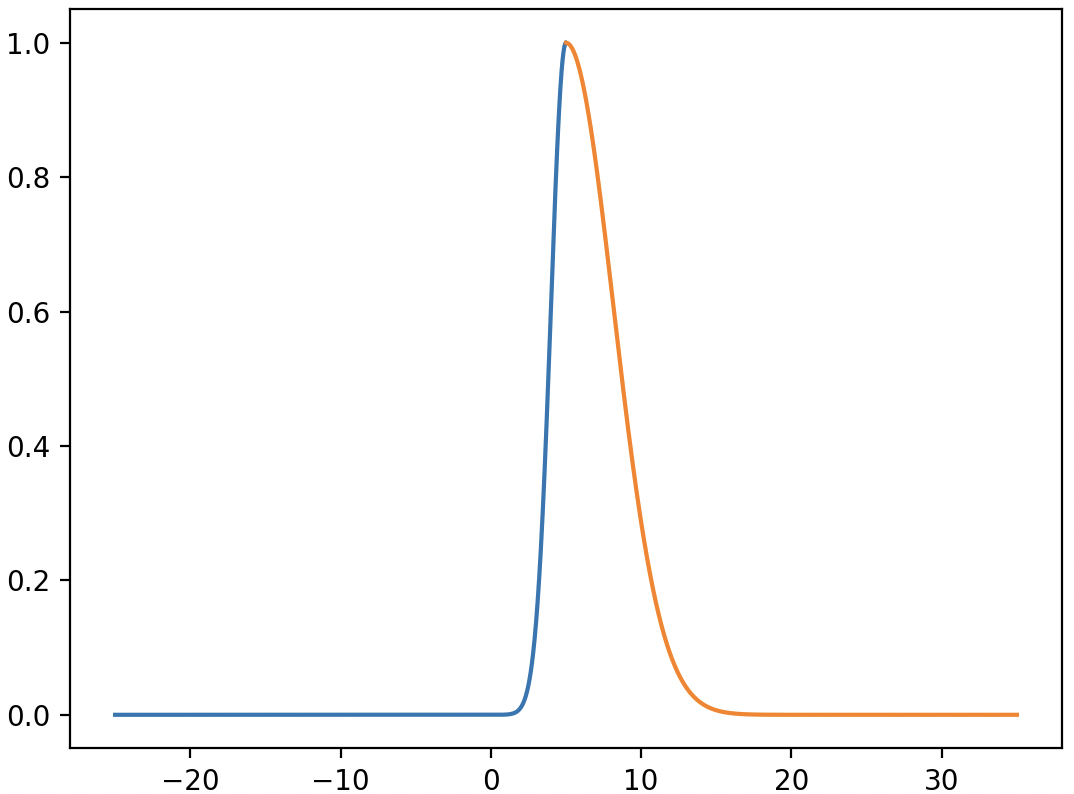
\includegraphics[width=0.9\textwidth]{../images/piece_gaussian.png}
		\end{center}
		\caption{分段高斯函数,$\theta_0=5, \sigma_1 = 1, \sigma_2 = 10$}
	\end{figure}

	该函数对小基线惩罚更大,夹角小于$5$度,走小方差分支,下降更快;大于5度,走大方差分支,下降平稳一些。\\

	最终图像对打分,
	$$
		s_{ij} = \sum_{\mathbf{p}}\mathcal{G}\left(\theta_{ij}(\mathbf{p})\right)
	$$

	匹配点对越多,且夹角不小于5度,则图像之间打分越高。

\subsection{实现细节}
	MVSNet将$1200 \times 1600$的原图下采样到$800 \time 600$,从中心crop出$512 \times 640$作为输入,经过特征提取后生成$128 \times 160 \times 32$的特征图。\\

	输出为参考图的深度值,GroundTruth也是参考图的深度值,均为$128 \times 160$。 处理分几个步骤,

	\begin{itemize}
		\item 每次输入3张图,一张为参考,2张目标,经过特征提取后,得到三个$128 \times 160 \times 32$的特征图
		
		\item 采用192个深度单位,通过单应变换将参考坐标变换到两个目标相机姿态下

			\textit{作者原始实现用了复杂的单应矩阵,非常繁琐;pytorch版本用了增广变换矩阵,非常简洁}

		\item 根据坐标变换得到两个$192 \times 128 \times 160 \times 32$的特征图,如上节描述

			\textit{按深度方向,从425mm到935mm,按2mm间隔离散成192个像平面}

		\item 连同参考特征图一起,计算三个\textbf{Feauture Volume}的方差,得到\textbf{Cost Volume};进行3D卷积,通过softmax沿着深度方向作概率归一化,结果为\textbf{Probability Volume},维度为$192 \times 128 \times 160$

		\item 沿\textbf{Probability Volume}深度方向计算深度期望值,得到维度为$128 \times 160$的深度特征图,
			$$
				D = \sum_{d = d_{min}}^{d_{max}} d \times \mathbf{P}(d)
			$$

			论文中提到,这一步实际想对\textbf{Probability Volume}作一个$\arg\max$操作,选出当前位置最可能的深度值,但是$\arg\max$无法求导,无法进行梯度回传,所以用soft $\arg\max$(原文说成是soft $\arg\min$)。

			\textit{所谓soft $\arg\max$实际就是利用了$softmax$逼近$\arg\max$的特性,以此来代替$\arg\max$\footnote{\url{https://en.wikipedia.org/wiki/Softmax_function}}}

		\item 通过$L_1$回归参考图的深度值;这里只有参考图的深度值为GroundTruth,src图的深度值未使用。
	\end{itemize}

	在增量SfM方法中,一次考虑所有图像,通过反投影距离进行优化,得到整个场景的点云;但在具体实现中,至少被三个相机看到的点,才能重建出点云;\\

	MVSNet中,训练的时候只是用了3张图片,但可以推断出参考图像上所有点的深度信息;在后处理时需要把图片两两输入,构建整个场景的点云。\\

	SfM的依赖图像之间的对应点对,具体会通过SIFT特征或深度学习的方法去构建对应关系;这一步实际也会引入很多匹配噪音,尤其对一些纹理较少的图像,能计算出的匹配点较少。\\

	MVSNet没有这一步处理,对应关系已经隐含在深度预测中,能匹配的点对,看到的深度也应该一样。\\

	事实证明,通过隐式特征构建对应关系,远远好于在RGB空间用显式特征构建对应关系。

\subsection{后处理}
	主要是对深度作两种过滤,

	\begin{itemize}
		\item \textbf{\textit{photometric约束}} \\

		对\textbf{Probability Volume}中概率小于0.8的点进行过滤;对噪音点不同的相机做出的判断方差会比较大,从而回归出的概率会变小

		\item \textbf{\textit{geometric约束}} \\
			
			点对$p,p^\prime$,以$p$图为参考图预测出深度值$d$;以$p^\prime$为参考图,预测出深度值$d^\prime$\\

			将$p^\prime$以深度$d^\prime$反投影到第一个视图,得到$p_{reproj}$,及对应的深度$d_{reproj}$

		\begin{align*}
			&\vert p - p_{reproj}| < 1\\
			&\frac{\vert d - d_{reproj}\vert}{d} < 0.01
		\end{align*}
		
		使得像素误差在1像素内,深度误差在1\%以内,文中提到这种约束至少在3视图上执行,如此同一点会有很多个重投影深度,取平均作为当前点的最终深度。
	\end{itemize}

\subsection{深度图融合}
	将不同视觉的深度图融合成场景点云,MVSNet采用“Real-time visibility-based fusion of depth maps”\footnote{\url{https://people.inf.ethz.ch/pomarc/pubs/MerrellICCV07subm.pdf}}的方法,看了下就是基于简单的遮挡规则来过滤一些不置信的点。\\

	这个文章也是作者的,虽然文中引用了自身,但code是在他人基础上改的,思路是下面第一篇。。。

	\begin{itemize}
		\item  Massively parallel multiview stereopsis by surface normal diffusion\footnote{\url{https://www.cv-foundation.org/openaccess/content_iccv_2015/papers/Galliani_Massively_Parallel_Multiview_ICCV_2015_paper.pdf}}
		\item Pixelwise view selection for unstructured multi-view stereo(COLMAP)\footnote{\url{https://demuc.de/papers/schoenberger2016mvs.pdf}}
		\item Structure-from-Motion Revisited\footnote{\url{https://openaccess.thecvf.com/content_cvpr_2016/papers/Schonberger_Structure-From-Motion_Revisited_CVPR_2016_paper.pdf}}
	\end{itemize}

	后两篇文章是COLMap的基础,MVSNet也有间接参考。

\subsection{问题\&改进}
	为什么要将场景切成192片,作单应变换去构建Cost,而不是直接通过基础矩阵变换构建Cost?\\

	单应变换是传统处理常用的手段,这个文章发表比较早,受传统MVS影响比较大,可能当时还没有建立端到端的思路,或者是端到端没做出效果。\\

	切片思路得假设目标场景最大最小距离,切片多了影响计算性能,并且有很多无意义的切片;切片少了又影响精度,对此"Cascade Cost Volume for High-Resolution Multi-View Stereo and Stereo Matching"\footnote{\url{https://arxiv.org/abs/1912.06378}}这个文章专门提了一些切片的优化方法,后面我们再细说。

\section{训练集结构}
	
	\subsection*{DTU数据集} 
		mvsnet用的是DTU数据集,DTU数据集通过移动的机械臂在$49$或$64$个位置,用$7$种光照,通过结构光扫描了$124$个场景,生成$1200 \times 1600$像素的图片及对应的点云信息。\\

		因此,每个场景有$49 * 7 = 343$张照片,整体数据集包含$42532$张照片及对应的点云信息。因为机械臂移动受到严格控制,所以每张图片都有对应的高精度相机参数。\\

		mvsnet训练集用了$79$个场景,共计$27097$张图片;测试集用了$22$个场景,共计$7546$张图片。
	
	\subsection*{深度信息}
		MVSNet的输入的是每个点的深度,通过泊松表面重建,将DTU数据集的点云转变为mesh,计算出每个像素点对应的深度信息。

	\subsection*{数据集结构}
		\begin{itemize}
			\item mvs{\_}training$\slash$dtu$\slash$Cameras$\slash$pair.txt 记录了$49$个位置,每个位置的照片与其他$10$张照片的匹配程度;注意这个pair内容与场景无关,仅与相机位置有关。因为相机位置受到精准控制,所以通过空间关系可以描述出位置之间的差异。

			\item mvs{\_}training$\slash$dtu$\slash$Cameras{\_}train$\slash$000000\{YY\}{\_}cam.txt 存放相机内外参数及尺度缩放信息

			\item mvs{\_}training$\slash$dtu$\slash$Rectified$\slash$scan\{XX\}{\_}train 训练样本,XX为场景编号
				\begin{itemize}
					\item rect{\_}0\{YY\}{\_}\{Z\}{\_}r5000 为场景scanXX对应的图片,YY为相机位置编号$ 1 \sim 49$,Z为光照强度编号$0 \sim 6$
				\end{itemize}

			\item mvs{\_}training$\slash$dtu$\slash$Depths$\slash$scan\{XX\}{\_}train$\slash$
				\begin{itemize}
					\item depth{\_} map{\_}00\{YY\}.pfm 场景scanXX对应相机位置YY($0 \sim 48$)的深度图,格式为pfm
					\item depth{\_} map{\_}00\{YY\}.png 深度图的可视化
				\end{itemize}
			
		\end{itemize}	

\bibliography{math}
\end{document}